\section{Results: Single-Antenna Devices}
\label{sec:results-single}

% src: seed_repeats_all_models_summary.json per_config.*_h0/_h5 runs (seed-paired single_mae differences)
For single-antenna devices in the macro-cell study, history produced no detectable change in error in any of the seven model families~(Figure~\ref{fig:history-gain-ci}). The seed-paired changes from $h=0$ to $h=5$ range from a $1.39\,\text{m}$ increase to a $0.32\,\text{m}$ decrease, and every confidence interval spans zero. The null result is tight where the measurement is precise: XGBoost's change is $0.06 \pm 0.18\,\text{m}$ on a baseline of $35.8\,\text{m}$, and Random Forest's is $0.32 \pm 0.86\,\text{m}$. The same seven models gained $15$ to $21\%$ on multi-antenna devices drawn from the same test users. Each split contains between $5$ and $10$ single-antenna test users, eight on average, which is why their confidence intervals are wider. With $50\%$ of the devices single-antenna, which gives $14$ to $22$ such test users per split, XGBoost shows a small gain after all, $0.30 \pm 0.24\,\text{m}$, and Random Forest none, $0.18 \pm 0.24\,\text{m}$. The accurate statement is that history gives these devices no more than about $1\%$ on uniform-NLOS data.
% src: diagnostics_2026_10/*/history_mechanism_diagnostic_summary.json user_counts (single-antenna test users per seed 42/1/7/13/99: 10, 7, 6, 10, 5; identical splits in both datasets)

% src: FINAL_REPORT.md §7.3 (outlier audit, 1D-CNN, single run: worst five all 1-antenna, best five all multi-antenna; user 250 raw MAE 33.84 m, Figure 6); diagnostics_2026_10/baseline_uniform_nlos/errors_first_seed.npz (seed 42, XGBoost: user 250 true bearing span 73 deg, predicted 17 deg at h=0 and h=5, range mean 94/96 vs 103 true; user 27 span 65 vs 68 deg); followup_2026_10/naive_baseline; single_share_50/uniform_nlos
The reason is visible in Section~\ref{sec:results-error-scale}: always predicting the mean training position gives $38.5\,\text{m}$ for these devices, so a snapshot model at $36.3\,\text{m}$ has recovered only about $6\%$ of it, and history leaves that unchanged. Figure~\ref{fig:trajectories} shows what the failure looks like for the median single-antenna test user. The user's walk spans $73^\circ$ of bearing, but the predicted positions, with or without history, span only $17^\circ$, at roughly the right distance from the BS (mean predicted range $96\,\text{m}$ against $103\,\text{m}$ true). This user is illustrative; over all single-antenna devices the predicted range correlates only $0.51$ with the true range. The median multi-antenna user's predictions instead follow the shape of the walk, spanning $68^\circ$ against $65^\circ$ true. This pattern dominates the tail of the error distribution: in a single-run audit of every test user, all five users with the largest error were single-antenna devices and all five with the smallest were multi-antenna devices.
% src: FINAL_REPORT.md §7.3 (outlier audit, 1D-CNN, single run)

\begin{figure}[h]
  \centering
  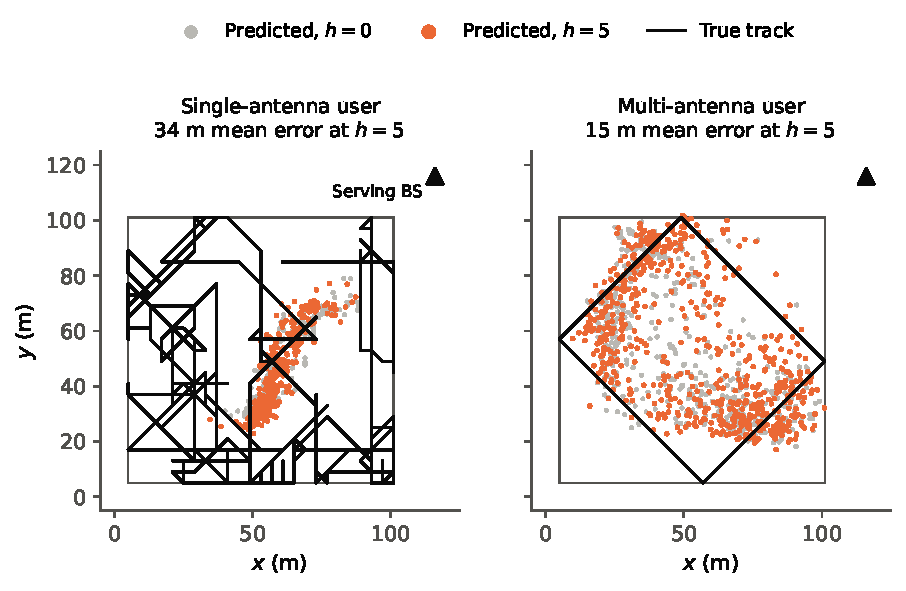
\includegraphics[width=0.92\textwidth]{fig_trajectories}
  \caption{True track and predicted positions of the median single-antenna~(left) and median multi-antenna~(right) test user, ranked by error at $h=5$. XGBoost without history~(gray) and with five steps of history~(orange), macro-cell study, one seed. The box marks the grid; the triangle marks the serving BS.}
  \label{fig:trajectories}
\end{figure}
% src: figure_scripts/make_figures_diagnostic.py trajectories(); diagnostics_2026_10/baseline_uniform_nlos/errors_first_seed.npz (seed 42; users 250 and 27, mean error at h=5 33.9 and 15.0 m)

% src: technical_documentation.md §7.4.1 (untuned, spherical: RF BASE 15.243 -> BASE_H3 18.057), §7.4.3 (tuned Cartesian: RF 14.022 -> 16.272; XGB 29.239 -> 13.430), §7.4.4 (block-shuffled: RF 13.811 -> 17.342; XGB 29.766 -> 14.800)
The single-user $25\times25$ regression runs point the same way at the same range, under a different split~(Figure~\ref{fig:single-user}). With RSS and SINR only, Random Forest's error rose when three steps of history were added, from $14.0$ to $16.3\,\text{m}$ under a chronological split and from $13.8$ to $17.3\,\text{m}$ when the walk was cut into shuffled five-step blocks to prevent any memorization of the path. XGBoost's error fell sharply with history in the same runs, but only from a snapshot model that was about twice as poor as Random Forest's, to roughly Random Forest's snapshot level. In none of these runs did a model with RSS and SINR history beat the best snapshot model by a margin worth reporting. Random Forest's loss is consistent with a feature-subsampling effect: replacing the stacked absolute lags with differences from the current snapshot removed it in a related configuration with AoA, and the macro-cell features already include such differences.
% src: technical_documentation.md §7.4.5 (hybrid delta features: RF 8.090 -> 7.636 m)

\begin{figure}[h]
  \centering
  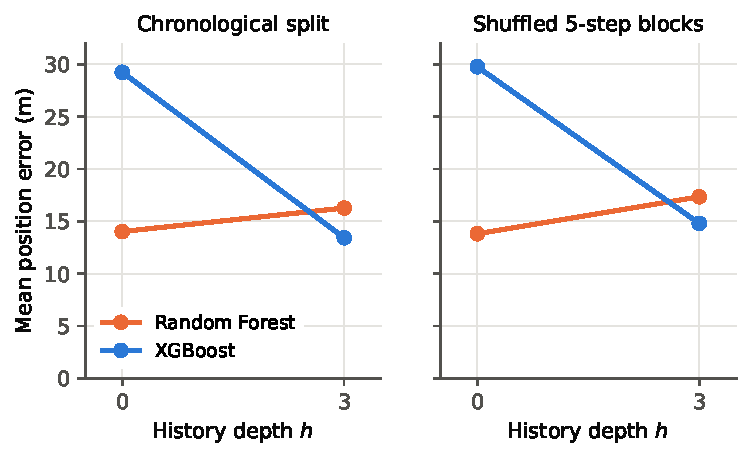
\includegraphics[width=0.7\textwidth]{fig_single_user_no_aoa}
  \caption{Single-user $25\times25$ regression with RSS and SINR only: mean position error without history and with three steps of history, under a chronological split~(left) and with the walk cut into shuffled five-step blocks~(right). Single run per point.}
  \label{fig:single-user}
\end{figure}
% src: figure_scripts/make_figures.py single_user_no_aoa(); technical_documentation.md §7.4.3, §7.4.4

% src: FINAL_REPORT.md §7.6 (1D-CNN masking: single 33.607 -> 32.188, multi 15.408 -> 15.279), §7.6.1 (k-NN/RF/XGB single: 39.968 -> 40.295, 33.069 -> 33.145, 34.806 -> 34.492; overall worse in all three); §5.7 significance table
How a missing angle is encoded does matter for one kind of model. Feeding single-antenna devices a dummy $0^\circ$ angle makes the derived channels assert a confident bearing, since $\cos 0^\circ = 1$. Replacing the angle embeddings with zeros, a point off the unit circle that no real angle can produce, and adding an explicit flag for angle validity lowered the 1D-CNN's single-antenna error from $33.6$ to $32.2\,\text{m}$ in a paired single-seed comparison, with a negligible $0.13\,\text{m}$ change for multi-antenna devices. The same encoding did not help $k$-NN, Random Forest or XGBoost, whose overall error rose slightly in all three cases. A tree can already branch on antenna count and ignore the angle channels when they carry nothing, whereas a convolution applies the same filters to every sample and cannot. The $1.4\,\text{m}$ improvement exceeds the paired uncertainty of the history comparison but lies within the seed-to-seed spread of the single-antenna error, so it is suggestive rather than established.

\subsection{A Range-Dependent Explanation}
\label{subsec:hypothesis}

% src (derived): pathloss_fit_summary.json range_resolution fitted_db_per_m (1.4176 dB/m at 10 m; 0.1487 dB/m at 95 m) x step length (2 m controlled grid; 4 m macro cell); sigma 10.1 dB; angular: 4 m / 95 m rad = 2.4 deg vs 4 deg Gaussian + 5 deg codebook (csi_dataset.py)
The contrast with the controlled grid, where RSS and SINR history did help, has a candidate explanation in Equation~(\ref{eq:rss-gradient}). Without an angle, a history window can only reveal motion through changes in RSS and SINR, and the change produced by one step shrinks with distance from the BS. With the fitted constants, a $2\,\text{m}$ step at $10\,\text{m}$ from the BS changes RSS by about $2.8\,\text{dB}$, whereas a $4\,\text{m}$ step at the macro cell's median range of $95\,\text{m}$ changes it by about $0.6\,\text{dB}$, almost five times less, against shadowing with a spread of $10\,\text{dB}$. An angle measurement weakens with range too, but far less severely relative to its noise: a $4\,\text{m}$ sideways step at $95\,\text{m}$ turns the bearing by about $2.4^\circ$, comparable to the $4^\circ$ angle error. On this account, history helps wherever the step-to-step change in some measured channel stands out from that channel's noise, which at macro range is true of the angle channels and not of RSS.

The account is a hypothesis. The controlled grid and the macro cell differ in other ways as well, most notably in testing seen rather than unseen users, so the range comparison between them cannot by itself isolate the mechanism. It does, however, make three predictions that can be tested within the macro-cell study alone, by feeding the models history for only one group of channels at a time on otherwise identical inputs. These predictions were fixed before that experiment was run. First, for multi-antenna devices, history of the angle channels should recover most of the full gain, and history of RSS and SINR alone should recover little of it. Second, for single-antenna devices, no subset of history should lower error beyond its confidence interval. Third, whatever gain RSS and SINR history does provide should be largest for devices closest to the BS and should fall with range.
